\section{拓扑排序}
\label{sec:graph-topological-order}

编译程序时，一个模块要等它引用的模块编译完才能编译；计算一组中间量时，一个量要等它依赖的量算出来才能计算。用有向图表示这类依赖，弧$u\to v$表示$u$必须先于$v$处理，问题就是把所有顶点排成一列，使每条弧的起点都排在终点前面。

\begin{definition}[拓扑序]
\label{def:graph-trav-topological-order}
有向图$\mathcal G=(V,E)$的\term{拓扑序}（topological order）是$V$中全部顶点的一个排列$v_1,v_2,\ldots,v_n$，使得对每条弧$v_i\to v_j$都有$i<j$。求拓扑序的过程称为拓扑排序。
\end{definition}

拓扑序只要求每条弧前后正确，没有弧相连的两个顶点谁先谁后都可以，因此拓扑序一般不唯一。但并非每个有向图都有拓扑序。若图中有有向环$v_1\to v_2\to\cdots\to v_k\to v_1$，排列既要让$v_1$在$v_2$之前、$v_2$在$v_3$之前……$v_{k-1}$在$v_k$之前，又要让$v_k$在$v_1$之前，这不可能。所以有拓扑序的图一定没有有向环。下面的Kahn算法会证明反方向也成立，从而得到：

\begin{theorem}[拓扑序的存在性]
\label{thm:graph-trav-topological-existence}
有限有向图存在拓扑序，当且仅当它是有向无环图。
\end{theorem}

必要性已在上面说明；充分性由下面算法~\ref{alg:graph-trav-kahn}的正确性给出。本节给出两种构造拓扑序的方法，它们在遇到有向环时都会报告失败，而不是输出一个不完整的序列。

\subsection{Kahn算法}
\label{sec:graph-trav-kahn}

\paragraph{当前入度与零入度队列}
哪个顶点可以最先处理？没有任何依赖的顶点，也就是入度为$0$的顶点。把它输出后，它对后继的约束就满足了，可以把它和它的出弧从图中删掉；删掉之后，有些原来有依赖的顶点会变成入度为$0$，可以接着输出。实现时不必真的删除，只需维护每个顶点在“尚未输出的顶点构成的子图”中的当前入度，并用一个队列存放当前入度为$0$、尚未输出的顶点。这一方法称为\term{Kahn算法}（Kahn's algorithm）。

\begin{algorithm}[Kahn拓扑排序]
\label{alg:graph-trav-kahn}
输入：有向图$\mathcal G=(V,E)$的出邻接表。输出：一个拓扑序，或报告图中有有向环。
\begin{enumerate}
  \item 扫描全部弧，统计每个顶点的入度$\operatorname{indeg}(v)$。把所有入度为$0$的顶点（包括孤立点）放入队列$Q$，输出序列$L$置空。
  \item 当$Q$非空时，取出队首$u$，追加到$L$末尾。对每条出弧$u\to v$，令$\operatorname{indeg}(v)\gets\operatorname{indeg}(v)-1$；若它恰好降为$0$，把$v$放入$Q$。
  \item $Q$为空时停止。若$L$含全部$n$个顶点，输出$L$；否则报告有有向环。
\end{enumerate}
\end{algorithm}

一个顶点只在当前入度刚降到$0$的那一刻入队，因此不会重复入队。判断必须用当前入度，而不是初始入度：初始入度为$1$的顶点，在它唯一的前驱输出之前不能输出。

\paragraph{为什么总能找到零入度顶点}
算法能一直进行下去，依赖于下面的事实。

\begin{lemma}[有向无环图有源点]
\label{lem:graph-trav-dag-source}
非空的有限有向无环图至少有一个入度为$0$的顶点。
\end{lemma}

\begin{proof}
假设每个顶点的入度都至少为$1$。从任一顶点$v_0$出发，取它的一个前驱$v_1$，即有弧$v_1\to v_0$；再取$v_1$的一个前驱$v_2$，如此继续。顶点只有有限个，这个序列中必有某个顶点第二次出现，设$v_i=v_j$，$i<j$。则$v_j\to v_{j-1}\to\cdots\to v_i$是一个有向环，与无环矛盾。
\end{proof}

由此可以证明算法的正确性。在有向无环图上，尚未输出的顶点构成原图的诱导子图，删掉顶点不会产生新的环，它仍是有向无环图；只要它非空，由引理~\ref{lem:graph-trav-dag-source}就有当前入度为$0$的顶点，这个顶点已经在队列中。因此队列在全部顶点输出之前不会变空，$L$最终含全部$n$个顶点。对每条弧$u\to v$，$v$的当前入度要等$u$输出后才扣除这条弧的贡献，所以$v$只能在$u$之后入队、之后输出，$L$满足拓扑序的要求。这就证明了定理~\ref{thm:graph-trav-topological-existence}的充分性。

反过来，若图中有有向环，环上每个顶点在环上都有一个前驱，环上第一个被输出的顶点在输出之前当前入度至少为$1$，不可能入队，所以环上的顶点一个也不会输出，$L$少于$n$个顶点。这时已经输出的部分只是一个前缀，不能当作完整的拓扑序。若需要给出环本身，可以在剩下的顶点中重复引理~\ref{lem:graph-trav-dag-source}证明中的“不断取前驱”，必然在有限步内回到已经走过的顶点，找到一个有向环。

\paragraph{菱形依赖的入度变化}
考虑弧为$1\to2$、$1\to3$、$2\to4$、$3\to4$的菱形依赖：任务$2,3$都依赖$1$，任务$4$同时依赖$2$和$3$。初始入度为$(0,1,1,2)$，只有$1$入队。图~\ref{fig:graph-trav-kahn}(b)列出了每次输出后的变化。输出$1$后，$2,3$的入度都降为$0$，两者入队；输出$2$后，$4$的入度从$2$降为$1$，还不能入队；输出$3$后，$4$的入度降为$0$，入队；最后输出$4$。得到拓扑序$1,2,3,4$。

\begin{figure}[!htb]
  \centering
  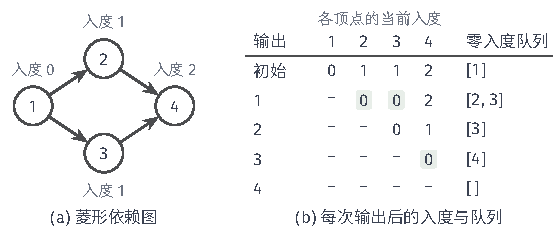
\includegraphics[width=94.8mm]{figures/01-basic-mathematics/04-graphs/tikz/c2-kahn-diamond/figure.pdf}
  \caption{Kahn算法在菱形依赖图上的执行。(a)依赖图及各顶点的初始入度。(b)每输出一个顶点后各顶点的当前入度（“--”表示已输出）与零入度队列；绿色底纹标出刚降为$0$、随即入队的入度。顶点$4$要等两个前驱都输出后才入队。}
  \label{fig:graph-trav-kahn}
\end{figure}

输出$1$之后，$2$和$3$同时位于队列中，这表示两项任务可以同时执行，或以任意先后执行。若先取$3$，就得到同样合法的$1,3,2,4$。队列中同时有多个零入度顶点时选哪一个，决定了得到哪个拓扑序。

\paragraph{计算开销}
统计入度要扫描每条弧一次；之后每个顶点入队、出队各一次，每条弧在其起点输出时被扣减一次。总时间为$O(n+m)$，入度数组、队列与输出序列占$O(n)$额外空间。若要求结果可复现，例如在多个零入度顶点中总是选编号最小的，就要把普通队列换成优先队列，每次入队、出队需要$O(\log n)$时间，总时间变为$O(m+n\log n)$。

\subsection{基于DFS的拓扑排序}
\label{sec:graph-trav-dfs-toposort}

\paragraph{逆完成次序}
第~\ref{sec:graph-trav-dfs-orders}节已经在一个例子中看到，把深度优先遍历的完成次序反转，弧的起点就排在了终点前面。下面说明这在无环图中总是成立。

\begin{theorem}[逆完成次序是拓扑序]
\label{thm:graph-trav-dfs-toposort}
对有向无环图执行一次覆盖全部顶点的深度优先遍历，则对每条弧$u\to v$都有$f(v)<f(u)$。因此按完成时刻从大到小排列顶点，得到一个拓扑序。
\end{theorem}

\begin{proof}
考察$u$检查弧$u\to v$的时刻，此时$u$处于处理中，按$v$的状态分三种情况。若$v$未发现，它将以$u$为父指针被发现，由引理~\ref{lem:graph-trav-dfs-nesting}，$f(v)<f(u)$。若$v$已完成，$f(v)$早于当前时刻，而$u$尚未完成，同样$f(v)<f(u)$。若$v$处于处理中，$u\to v$是一条回边，由定理~\ref{thm:graph-trav-directed-cycle}图中有有向环，与假设矛盾，这种情况不会发生。
\end{proof}

于是得到第二种构造：执行覆盖全部顶点的三色深度优先遍历；一旦遇到回边，就沿父指针返回一个有向环，拒绝输出排序；若始终没有回边，把完成次序反转后输出。实现时可以在每个顶点完成时把它放到输出序列的最前面，遍历结束时序列就已是逆完成次序。

\paragraph{与Kahn算法的结果比较}
在同一个菱形依赖图上，从$1$出发、按编号读取出邻居：发现$1,2,4$，$4$完成，$2$完成；回到$1$后发现$3$，$3$的出邻居$4$已完成，$3$完成；最后$1$完成。完成次序为$4,2,3,1$，反转得$1,3,2,4$，见图~\ref{fig:graph-trav-dfs-toposort}。它与Kahn算法给出的$1,2,3,4$不同，但两者都是合法拓扑序：把顶点按次序从左到右排开，四条弧全部指向右方。拓扑序可能不唯一，检验一个输出是否正确，标准是逐条弧核对先后，而不是与某一个特定答案比较。

\begin{figure}[!htb]
  \centering
  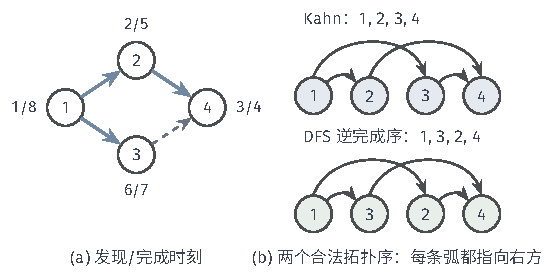
\includegraphics[width=93.8mm]{figures/01-basic-mathematics/04-graphs/tikz/c2-dfs-topological-order/figure.pdf}
  \caption{基于深度优先遍历的拓扑排序。(a)菱形依赖图上从$1$出发的深度优先遍历，旁注为发现/完成时刻，蓝色箭头为父指针对应的弧，虚线弧$3\to4$检查时$4$已完成。(b)Kahn算法得到的$1,2,3,4$与逆完成次序$1,3,2,4$，两种排列下每条弧都从左指向右，都是合法拓扑序。}
  \label{fig:graph-trav-dfs-toposort}
\end{figure}

\paragraph{必须覆盖全部顶点}
只从一个起点遍历时，得到的只是它可达部分的完成次序。在菱形图中若只从$2$出发，只能到达$2,4$，反转后是$2,4$，漏掉了$1$和$3$。也不能把各次重启的结果分别反转后简单拼接：先从$2$出发得到$2,4$，再从$1$出发得到$1,3$，拼成$2,4,1,3$，违反了弧$1\to2$。正确做法是把整次遍历的完成次序$4,2,3,1$作为一个整体反转，得到$1,3,2,4$；定理~\ref{thm:graph-trav-dfs-toposort}的证明对跨越不同起点的弧同样成立。

\paragraph{两种方法的选择}
两种方法的时间都是$O(n+m)$。Kahn算法显式地维护“当前可以执行的任务”这一集合，适合需要逐步列出可并行任务、或按某种优先规则选择任务的场合。基于深度优先遍历的方法不需要入度数组，在已经要做深度优先遍历、或需要在有环时给出环的场合可以直接复用同一次遍历。对一般有向图，可以先用第~\ref{sec:graph-trav-scc}节的方法求出强连通分量并缩点，再对无环的缩点图做拓扑排序。第~\ref{sec:graph-shortest-paths}节在有向无环图上计算最短路时，就是按拓扑序逐个处理顶点。
